\documentclass[../../main.tex]{subfiles}
\begin{document}


{\bf [解]} 

簡単のため$c = \cos x, s = \sin x$ とおく. 
また $p = s+c$ とすると 
\begin{align}
 sc = \dfrac{p^2-1}{2}, -\sqrt{2} \leqq p \leqq \sqrt{2} \label{eq:1}
\end{align}
である．$f(x)$を$s,c$のみで表すと
\begin{align}
f(x)  &= 3(s-c) - \cos 2x = 3(s-c) - (c^2-s^2) = (s-c)(s+c+3)  \label{eq:2}
\end{align}
だから，一階微分は
\begin{align}
 f'(x) 
&= 3(c+s) + 2\sin 2x \\
&= 3(c+s) + 4sc \\
&= 3p + 2p^2 - 2 \\
&= (2p-1)(p+2)
\end{align}
である．よって\cref{eq:1}と合わせて増減表は以下のようになる．

\begin{table}[htb]
\centering
\caption{$f$の増減表．$\alpha, \beta$ は $p = \dfrac{1}{2}$ となるもの.}
\begin{tabular}{c|c*6{c}|c}
$x$ & $0$ & $\dots$ & $\alpha$ & $\dots$ & $\beta$ & $\dots$ & $2\pi$ \\ \hline
$p$ & $1$ & $+$ & $1/2$ & $-$ & $1/2$ & $+$ & $1$ \\ \hline
$f'$ & & $+$ & $0$ & $-$ & $0$ & $+$ & \\ \hline
$f$ & $-4$ & $\nearrow$ & & $\searrow$ & & $\nearrow$ & $-4$
\end{tabular}
\end{table}
よって求める最大小値は$f(\alpha), f(\beta), -4$のいずれかなので以下これを計算する．
\cref{eq:2}より$c-s$を評価しよう．

\begin{figure}[htb]
\begin{center}
\begin{tikzpicture}[scale=1.1, >=stealth]
  % 座標軸
  \draw[->] (-0.3, 0) -- (6.8, 0) node[below] {$x$};
  \draw[->] (0, -1.8) -- (0, 1.8) node[left] {$y$};

  % 1. p = s + c = sin(x) + cos(x) (太い実線・青)
  \draw[domain=0:6.283, samples=100, smooth, thick, blue!80!black] 
      plot (\x, {sin(\x r) + cos(\x r)}) 
      node[right, font=\small] {$p = s+c$};

  % 2. s - c = sin(x) - cos(x) (破線・赤)
  \draw[domain=0:6.283, samples=100, smooth, thick, dashed, red!80!black] 
      plot (\x, {sin(\x r) - cos(\x r)}) 
      node[right, font=\small] {$s-c$};

  % 基準線 y = 1/2
  \draw[dashed] (0, 0.5) node[left, font=\small, black] {$\dfrac{1}{2}$} -- (6.0, 0.5);

  % 基準線 y = 0 の補助（x軸上の境界点）
  % s - c = 0 の交点: x = pi/4, 5pi/4
  \fill[red!80!black] (0.785, 0) circle (1.5pt);
  \fill[red!80!black] (3.927, 0) circle (1.5pt);

  % α, β のプロットと垂直点線
  \draw[dashed] (2.05, 0.5) -- (2.05, 0) node[below, font=\small] {$\alpha$};
  \draw[dashed] (5.80, 0.5) -- (5.80, 0) node[below, font=\small] {$\beta$};

  % α, β における s - c の値を強調マーク
  \fill[purple] (2.05, {sin(2.05 r) - cos(2.05 r)}) circle (1.5pt) 
      node[above left, font=\scriptsize] {$s-c > 0$};
  \fill[purple] (5.80, {sin(5.80 r) - cos(5.80 r)}) circle (1.5pt) 
      node[below left, font=\scriptsize] {$s-c < 0$};

  % 主な x 軸ラベル
  \node[below, font=\scriptsize] at (0.785, 0) {$\dfrac{\pi}{4}$};
  \node[below, font=\scriptsize] at (3.927, 0) {$\dfrac{5\pi}{4}$};
  \node[below right, font=\small] at (6.28, 0) {$2\pi$};
  \node[below left, font=\small] at (0, 0) {$0$};

\end{tikzpicture}
\end{center}
\caption{$p = s+c$（実線）と $s-c$（破線）のグラフ，および $\alpha, \beta$ における符号関係}
\end{figure}

\cref{eq:1}より
\begin{align}
s-c &= \pm \sqrt{(s-c)^2} = \pm \sqrt{(s+c)^2 - 4sc} \\
&= \pm \sqrt{2-p^2}
\end{align}
である．また図より $x=\alpha$ の時 $s-c > 0$, $x=\beta$ の時 $s-c < 0$ だから
\begin{align}
\begin{cases}
f(\alpha) = \sqrt{2-\dfrac{1}{4}} \left( \dfrac{1}{2} + 3 \right) = \sqrt{2-\dfrac{1}{4}} \cdot \dfrac{7}{2} = \dfrac{7}{4}\sqrt{7} \\
f(\beta) = -\sqrt{2-\dfrac{1}{4}} \left( \dfrac{1}{2} + 3 \right) = -\sqrt{2-\dfrac{1}{4}} \cdot \dfrac{7}{2} = -\dfrac{7}{4}\sqrt{7}
\end{cases}
\end{align}
となる．端点での値$-4$と比べると $-4 > -\dfrac{7}{4}\sqrt{7}$ だから求める最大最小値は
\begin{align}
\text{max} \;\; \dfrac{7}{4}\sqrt{7}, \quad \text{min} \;\; -\dfrac{7}{4}\sqrt{7}
\end{align}

\end{document}
OB